%% $Id: techspec.tex,v 1.5 2000/05/14 23:09:32 matt Exp $

\chapter{Specification and Design}
\label{techspec}
This chapter details the final specifications for the components needed for OSDigger to function.

\section{Overall Design}

The overall design here has been expanded from the initial design to take into account the results from the research into related work and the prototype.  One of the main changes has been the split of the indexer into two halves: the \emph{indexer} and the \emph{inverter}.  

\begin{figure}[htbp]
  \begin{center}
    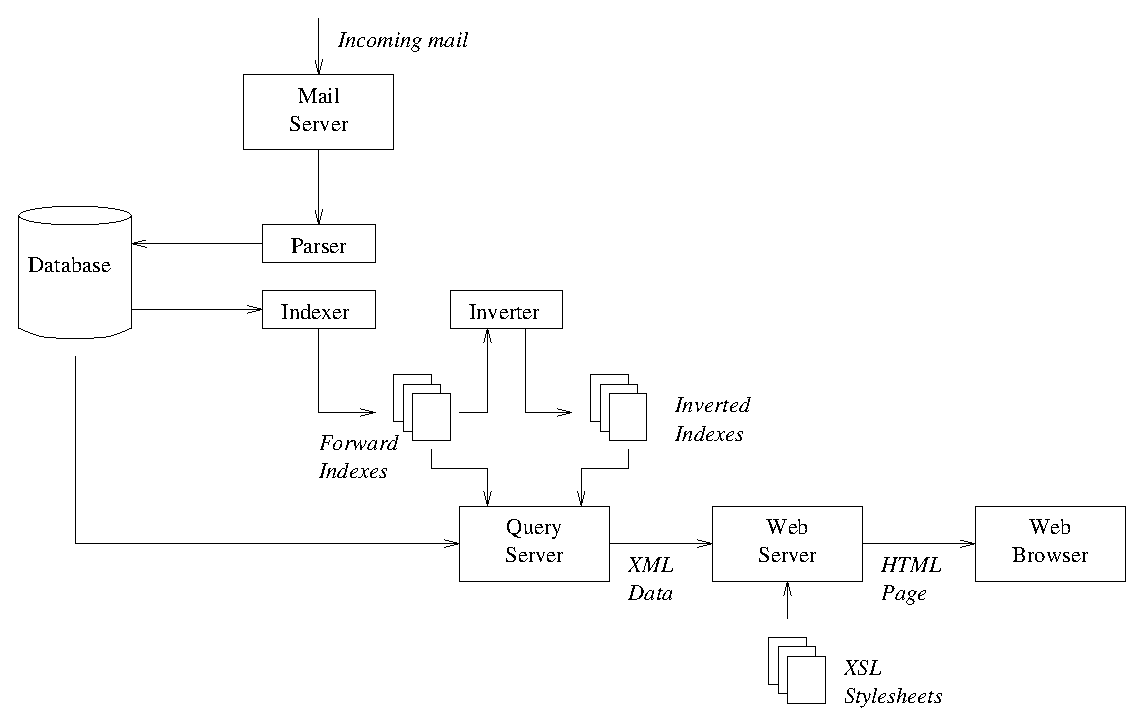
\epsfig{file=figures/dataflow.eps,width=12cm}
    \caption{Data flow in OSDigger}
    \label{fig:dataflow}
  \end{center}
\end{figure}

The flow of data through the system is shown in Figure \ref{fig:dataflow}.  Note that the web server communicates directly with the Query server, and not the Database server.  This is to reduce the number of communication paths in the system.  Also note that all information passed from the Query server to the Web server is encoded in XML.

\section{Database}
\label{sec:db}
MySQL will be used as the database to store the messages.  The messages will be parsed by a perl script called from the mail server and inserted into the \texttt{messages} table of the database.  The \emph{To}, \emph{from}, \emph{subject}, \emph{cc}, \emph{date}, \emph{message-id}, and \emph{in-reply-to} or \emph{references} headers are all stored as separate fields in the database.  The table scheme is shown in Table \ref{tab:messages}.

\begin{table}[htbp]
  \begin{center}
    \begin{tabular}{|l|l|l|l|l|l|}
\hline
Field       & Type             & Null & Key & Default     & Extra           \\
\hline
\hline
id          & int(10) unsigned &      & PRI & 0           & auto\_increment  \\
hmessage\_id & varchar(255)     &      & MUL &            &                 \\
hrefs        & varchar(255)     &      & MUL &            &                 \\
hdate       & datetime         &      & MUL & 0000-00-00  &                 \\
hsubject    & varchar(255)     & YES  &     & NULL        &                 \\
hfrom       & varchar(255)     & YES  &     & NULL        &                 \\
hto         & varchar(255)     & YES  &     & NULL        &                 \\
hcc         & varchar(255)     & YES  &     & NULL        &                 \\
list        & int(10) unsigned &      & MUL & 0           &                 \\
body        & text             & YES  &     & NULL        &                 \\
\hline

    \end{tabular}
    \caption{\texttt{messages} table scheme}
    \label{tab:messages}
  \end{center}
\end{table}

The message bodies are to be compressed/decompressed by a User Defined Function (UDF) using the zlib compression library. 

An additional table \emph{lists}, Table \ref{tab:lists} stores information about the lists themselves, such as the list number, subscription address, posting address, type.


\begin{table}[htbp]
  \begin{center}
    \begin{tabular}{|l|l|l|l|l|l|}
\hline
Field       & Type             & Null & Key & Default     & Extra           \\
\hline
\hline
listnum    & int(10) unsigned &      & PRI & 0   &   \\
subaddr    & varchar(255)     &      &     &     &   \\
addr       & varchar(255)     &      &     &     &   \\
type       & int(11)          &      &     & 0   &   \\
\hline

    \end{tabular}
    \caption{\texttt{lists} table scheme}
    \label{tab:lists}
  \end{center}
\end{table}

\section{Indexer}
The indexer is to be split into two parts.  The \emph{indexer} and the \emph{inverter}.  Both are to be written in C.

\subsection{Indexer}
The indexer is to extract the message bodies, address and subject fields from the database using the MySQL C API.  The indexer should then parse the message text and stem all words using the Porter Stemming algorithm \cite{porter80}.  The words in each document are then looked up in the lexicon to find their wordids.  Words not found in the lexicon are added.  Each time a word is looked up a count of the number of occurrences of that word in the lexicon should be incremented.

The words are partitioned into 8 sets using the first 3 bits of their wordid.  Each set is sorted into ascending order then stored as a compressed list using the Local Bernoulli method with Golomb coding as described in Section \ref{compression}.  The local parameter $d$ is calculated as

\[
0.69 \times \frac{\textrm{the total number of words in the lexicon}}{\textrm{the number of words in the list}}
\]

and stored at the start of each list, along with the number of words in that list.  The format of each record is shown in Figure \ref{fig:forward}.

Each time the indexer is run, it must append the new messages in the database to the end of the existing forward indexes.

\subsection{Inverter}
The inverted takes each one of the forward indexes in turn and inverts it into an inverted index.  The inversion is to take place in memory.  The inverted indexes are to be stored in BerkeleyDB databases with the wordid in the key.  The number of documents, the local Bernoulli parameter $d$ and the compressed list of document numbers are stored as the value.  The format is shown in Figure \ref{fig:inverted}.

The inverter should replace each existing entry in the database with the updated version whenever it is run.

\section{Query Server}
\label{sec:qs}
The Query server is to be written in C.  It is a daemon process that listens on TCP port 3333.  The daemon uses a simple protocol to communicate with the web server.  The web server can issue one of three requests:

\begin{center}
\begin{tabular}{l|p{7cm}}
\emph{Command}  &  \emph{Description} \\
\hline
\texttt{onestep} \emph{start} \emph{num} \emph{term} [\emph{term} ...] & Perform a onestep search and return \emph{num} results starting from \emph{start} in XML \\
\texttt{twostep} \emph{term} [\emph{term} ...] & Perform a twostep search and return the results in XML \\
\texttt{retrieve} \emph{docid} & Fetch a message and return it encoded in XML \\
\end{tabular}
\end{center}

The server computes the results for the queries passed to it.

\subsection{Onestep Queries}
To compute a onestep query, the server first stems the query terms and looks up the corresponding wordid from the lexicon.  It then retrieves the compressed list of document numbers from the appropriate inverted index for the word.  The lists are then decompressed and ranked together using the Cosine Ranking rule.  The resulting scores are sorted and \emph{num} results are returned starting at \emph{start}.

\subsection{Twostep Queries}
To compute a twostep query, the server first proceeds as a onestep query and returns the top 15 documents.  The documents are then looked up in the forward indexes to find out which words occur in them.  A tally is kept of each word and how often it appears.  The final tally is then multiplied by the TF$\times$IDF value for that word and the resultant scores sorted.  The server then returns the top 20 words.


\section{Web Site}
The interaction between the user and the query server is via a Java Servlet.  Hence the web server must support servlets.  The servlet will be responsible for taking the input from the user and formatting it and sending the query to the query server.  The format of the queries is described in Section \ref{sec:qs}.  

The servlet will take the XML data returned by the query server and apply an XSLT stylesheet (see Section \ref{sec:ui} to convert it to the desired output format (initially HTML, but other formats may follow).  The servlets is also responsible for handling any customisation the user wants.  This will be done by storing preferences in a MySQL database, keyed by an HTTP cookie, held by the users browser.

\section{Parser}
The parser will be written in Perl and will take messages passed to it from the mail server and parse them.  Any non-text MIME parts will be discarded, uuencoded and Base64 text parts will be decoded and converted to the host character set.

The message will then be inserted into the database and compressed using a User Defined Function in the database.  The headers of the message will be parsed and inserted as fields described in Section \ref{sec:db}.

% LocalWords:  OSDigger htbp dataflow eps XML MySQL perl int PRI hmessage MUL
% LocalWords:  varchar hrefs hdate hsubject hfrom hto hcc UDF zlib listnum addr
% LocalWords:  subaddr API wordids wordid Golomb BerkeleyDB onestep num twostep
% LocalWords:  docid TF IDF Servlet servlets servlet XSLT stylesheet HTML HTTP
% LocalWords:  uuencoded
